\section {Carboxylic Acid Orientation}

The orientation and geometry of succinic acid with respect to its position relative to the water surface was calculated. Figure \ref{fig:angle-definitions} depicts the succinic acid molecule and shows two angle definitions relative to the surface normal vector (labeled ``z''). The angular tilt, $\theta$, is an angle between the O-C-O bisector axis of the carboxylic acid head group (pointing from the carbon to the oxygen end) and the vector normal to the plane of the water surface. $\theta$ varies from being aligned with the surface normal ($\theta=0^{\circ}$), to perpendicular and in the plane of the surface ($\theta=90^{\circ}$), to anti-aligned with the surface normal ($\theta=180^{\circ}$). 

The carboxylic acid group twist angle, $\phi$, measures the angle between the plane formed by the O-C-O atoms of the carboxylic acid, and the plane formed by the O-C-O bisector and the surface normal vectors. This is the same as a dihedral angle defined by the following three vectors: surface normal (``z''), the O-C-O bisector axis, and the vector from the carbonyl carbon to the carbonyl oxygen of the acid group. Because of the symmetry of rotations about the carboxylic acid O-C-O bisector axis with respect to the plan of the water surface, $\phi$ has a range of $0^{\circ} \le \phi \le 180^{\circ}$. If $\phi=0^{\circ}$ the vector from the carbonyl carbon to the carbonyl oxygen is aligned in a plane perpendicular to the water surface, and pointing out of the surface. Consequently, the bond from the carbonyl carbon to the alcohol oxygen points towards the water bulk and lays in the same plane. A twist of $\phi=90^{\circ}$ places both the carbonyl and alcohol oxygens in the plane of the water surface. $\phi=180^{\circ}$ aligns the O-C-O plane similarly to $\phi=0^{\circ}$, but with the carbonyl carbon and alcohol oxygen bond pointing out from the water surface, and the carbonyl oxygen pointing in towards the water bulk. 

A third angle, $\psi$ (not shown), is the dihedral angle of the carbon backbone, where $\psi = 0^{\circ}$ turns the succinic acid into a ``trans-'' carbon-chain configuration. Symmetry of rotations limits the range of dihedral twists to $0^{\circ} \le \psi \le 180^{\circ}$.

%$0^{\circ} \le \theta \le 180^{\circ}$). 

\begin{figure}[h!]
	\begin{center}
		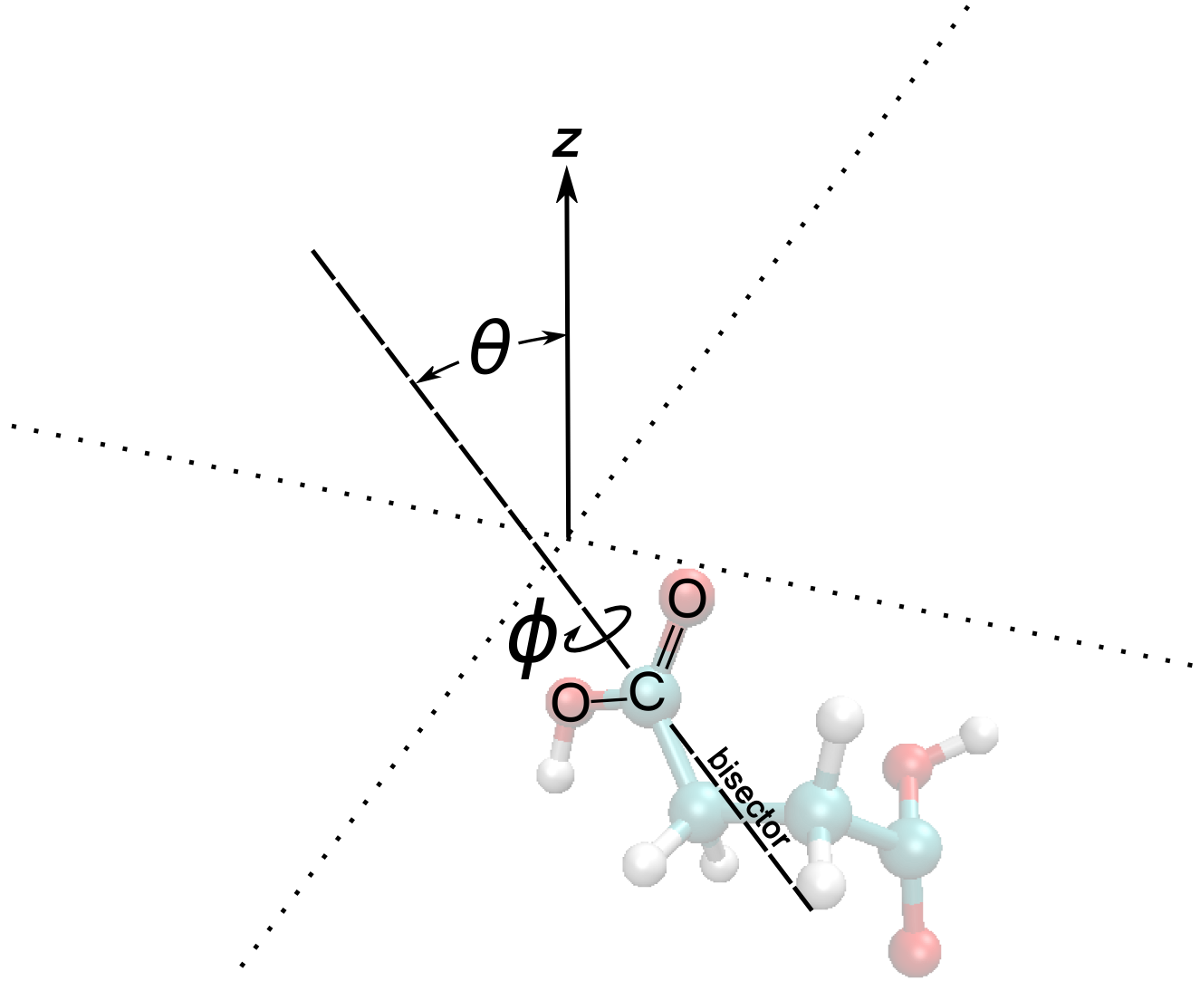
\includegraphics[scale=1.0]{images/bond-angles/bond-angle-definitions-small.png}
		\caption{Two angle definitions that characterize the carboxylic acid head group orientation relative to the water surface. The acid tilt, $\theta$, measures an angle formed between the O-C-O bisector axis of the acid group, and the vector normal to the plane of the water surface. Acid twist, $\phi$, is calculated as a dihedral formed by three vectors: the vector normal to the water surface, the O-C-O acid group bisector vector, and the vector pointing from the carbonyl carbon to the carbonyl oxygen.}
		\label{fig:angle-definitions}
	\end{center}
\end{figure}

We first look at the dihedral angle, $\psi$, to understand the orientation of the carbon backbone at different locations throughout the interface. Figure \ref{fig:dihedral} is an angular depth profile of the dihedral angle, $\psi$, on the y-axis, plotted against the distance of the molecular center of mass to the water surface, on the x-axis. Positions further into the water bulk appear on the left of the plot. The coloration ranges from dark blue to red, indicating low and high intensities of the 2D histogram, respectively. The greatest contribution is from the gauche configure of the acid groups. Clearly the molecule mostly has a $\psi$ value centered at $60^{\circ}$ at all depths, as indicated by the bright red streak running horizontally across the plot, centered at $\psi=60^{\circ}$. There are minor contributions from the cis-configuration of the carbon backbone at $\psi = 180^{\circ}$. The $180^{\circ}$ configuration is represented throughout the deeper regions of the interface and in the water bulk. Near -2\angs~and further towards the surface near 0\angs, the distribution completely shifts to the $60^{\circ}$ gauche configuration. The succinic acid molecules within approximately 2\angs of the surface location have a strong preference for a gauche dihedral configuration. 

\begin{figure}[h!]
	\begin{center}
		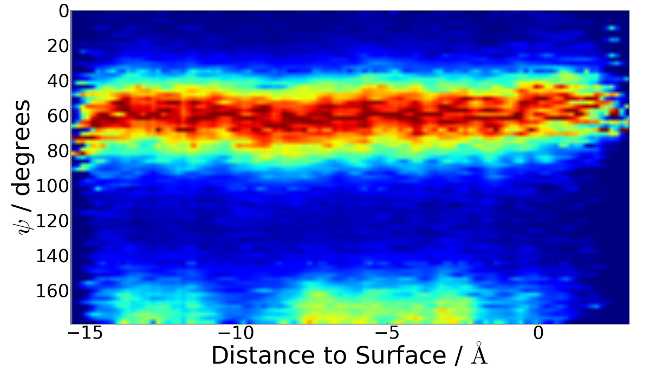
\includegraphics[scale=1.0]{images/dihedral/dihedral-small.png}
		\caption{The dihedral angle of the carbon backbone of the succinic acid molecule is found in either a gauche or cis- configuration. This angular depth profile shows the distribution of $\psi$ at different positions within the water interface. Dark blue and bright red coloration indicate low and high intensities of the histogram, respectively. The long streak of red centerd at $\psi=60^{\circ}$ shows the preference of the molecule to take on a gauche configuration throughout all depths from the water surface.}
		\label{fig:dihedral}
	\end{center}
\end{figure}


% Tilt/Twist
\begin{figure}[h!]
	\begin{center}
		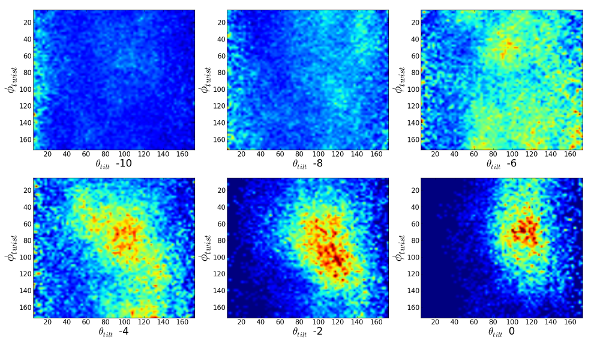
\includegraphics[scale=1.0]{images/bond-angles/carbonyl-tilt-twist-small.png}
		\caption{The tilt and twist of the carboxylic acid headgroups of the succinic acid ($\theta$ and $\phi$, respectively) characterize the orientation of the acid moiety relative to the water surface. Shown are several two-dimensional histograms of $\phi$ vs $\theta$ calculated at different depths of the interface. The depth value is calculed from the molecular center of mass, and the plots represent 2\angs~position slices along the water surface normal. The plots begin at -9\angs (
		\label{fig:tilt-twist}
	\end{center}
\end{figure}
